\documentclass[twosided,a4,10pt]{article}
\usepackage[utf8]{inputenc}
\usepackage{amsmath}
\usepackage{amsfonts}
\usepackage{amssymb}
\usepackage{amstext}
\usepackage{mathrsfs}
\usepackage{textcomp}
\usepackage{german}
\usepackage{graphicx}
\usepackage[usenames,dvipsnames]{xcolor}
\usepackage{pifont}
\usepackage{nicefrac}
\usepackage{sectsty}
\usepackage{dblfnote}
\usepackage{verbatim}
% ------
% Fonts and typesetting settings
\usepackage[sc]{mathpazo}
\usepackage[T1]{fontenc}
\linespread{1.1} % Palatino needs more space between lines
\usepackage{microtype}
\subsectionfont{\fontsize{10}{15}\selectfont}

% ------
% Page layout
\usepackage[hmarginratio=1:1,top=32mm,columnsep=20pt]{geometry}
\usepackage[font=it]{caption}
\usepackage{paralist}
\usepackage{multicol}

%--------
%Footnote
\usepackage{footnote}
\usepackage{perpage} %the perpage package
\MakePerPage{footnote} %the perpage package command
\addtolength{\skip\footins}{2pc plus 5pt}
%------
%caption hack
\usepackage{caption}

%\DeclareCaptionType{faltung}[][List of equations]
%\captionsetup[faltung]{labelformat=empty}

% ------
% Abstract
\usepackage{abstract}
\renewcommand{\abstractnamefont}{\normalfont\bfseries}
\renewcommand{\abstracttextfont}{\normalfont\small\itshape}


% ------
% Titling (section/subsection)
\usepackage{titlesec}
%\renewcommand\thesection{\Roman{section}}
\titleformat{\section}[block]{\large\scshape\centering}{\thesection.}{1em}{}

% ------
% Clickable URLs (optional)
\usepackage[hyphens]{url}
\usepackage{hyperref}

% ------
% Header/footer
\usepackage{fancyhdr}
\pagestyle{fancy}
%	\fancyhead{}
%	\fancyfoot[C]{WIS WS 2017/18 $\cdot$
% Software Engineering $\cdot$ Prof. Dr. Dünnweber}
\fancyhead[R]{OTH Regensburg $\cdot$ Fakultät IM}
%	\fancyfoot[RO,LE]{\thepage}
\fancyfoot[L]{WIS $\cdot$ WS 2017/18}
\fancyfoot[R]{Prof. Dr. Dünnweber}
\fancyfoot[C]{\thepage}


% ------
% Maketitle metadata
\title{\vspace{-5mm}%
	\fontsize{20pt}{10pt}\selectfont
	\textbf{Inhaltsbasierte Musikempfehlung mit Convolutional Neuronalen Netzwerken}
}	
\vspace{-5mm}\date{}
\author{
	\large\begin{minipage}[t]{0.5\linewidth}
		\begin{center}
			\textsc{Weidhas Philipp}\\[2mm]
			\normalsize	Matr.nr: 123456\\
			\normalsize
			\href{mailto:philipp.weidhas@st.oth-regensburg.de}
			{philipp.weidhas@st.oth-regensburg.de}
		\end{center}
	\end{minipage}
	\begin{minipage}[t]{0.5\linewidth}
		\begin{center}
			\textsc{Wildgruber Markus}\\[2mm]
			\normalsize	Matr.nr: 123456\\
			\normalsize
			\href{mailto:markus.wildgruber@stud.oth-regensburg.de}
			{markus.wildgruber@stud.oth-regensburg.de}
		\end{center}
	\end{minipage}
}




%%%%%%%%%%%%%%%%%%%%%%%%
\begin{document}
	\maketitle
	\thispagestyle{fancy}
	\begin{multicols}{2}
		\begin{abstract}
			\noindent Hier kommt die Zusammenfassung...
		\end{abstract}
		\section{Einleitung}
		Im ersten Halbjahr des Jahres 2017 wurden 62\% der Einnahmen der amerikanischen Musikindustrie durch Streaming Plattformen\footnote[1]{wie Spotify, Apple Music, Pandora etc.} erzielt. Im Vergleich zu Vorjahr erhöhten sich dadurch die Einnahmen um 48\% auf 2.5\$ Milliarde \cite{friedlander}. Dieser Erfolg basiert nicht nur auf einer guten Verfügbarkeit der Lieder und einem günstigen Preis sondern auch auf automatischen Musikempfehlungsdiensten, welche dem Nutzer ein angenehmeres Konsumverhalten ermöglichen.\newline
		Obwohl Empfehlungsdienste in den letzten Jahren viel erforscht wurden, ist das Problem der Musikempfehlung sehr komplex. Neben einer großen Anzahl an verschiedenen Stile und Genres, beeinflussen sowohl soziales- und geographisches Umfeld, sowie der aktuelle Gemütszustand die Vorliebe eines Hörers. Diese Aspekte müssen in einem Musikvorschlag berücksichtigt werden. \cite{oord}\newline
		Neben der Empfehlung bestimmter Lieder sollen Empfehlungssysteme zusätzlich noch das Cold-Start Problem sowohl bei einem Benutzer\footnote[2]{New User Problem (NUP)} als auch bei einem Lied\footnote[3]{New Song Problem (NSP)} überwinden. Das Cold-Start Problem besteht darin, dass noch keine Bewertungen für ein Lied vorliegen, wodurch es auch nicht vorgeschlagen werden kann. Dasselbe Problem gibt es bei einem neuen Benutzer: diesem kann kein guter Vorschlag gemacht werden, da es an Information mangelt welche Art von Musik ihm gefällt. \cite{celma}\\
		Mit Hilfe von Convolutional Neuronalen Netzwerken (CNN) können noch nicht alle Probleme überwunden werden, aber sowohl das NSP als auch die Empfehlung werden durch die Verwendung eines CNN als Empfehlungssystem verbessert.\newline\\
		Der weitere Verlauf der wissenschaftlichen Arbeit ist wie folgt organisiert. Im 2. Abschnitt werden die Grundlagen der Musikempfehlung vorgestellt. Im 3. Kapitel wir der Aufbau von Neuronale Netze, soweit zwei Neuronale Netze für inhaltsbasierte Musikempfehlung beschrieben. Im letzten Abschnitt schließt diese Arbeit mit einem Vergleich der Ergebnisse der beiden Modelle.
		TODO
		\section{Grundlagen der Musikempfehlung}
		In dem Gebiet des Musik Information Retrieval (MIR) gibt es vier Kategorien \cite{schedl} die einen Einfluss auf die Wahrnehmung von ähnlicher Musik haben.\newline \textit{Musikmerkmale} sind Eigenschaften, welche aus dem Audiosignal eines Liedes extrahiert werden. Dazu zählen Aspekte wie der Rhythmus, die Melodie, die Harmonie oder die Stimmung eines Stücks.\newline
		Als \textit{Musikkontext} versteht man alle Aspekte, die nicht aus dem Audiosignal abgeleitet werden, sondern Informationen die über ein Musikstück bekannt sind. Beispielsweise Metadaten wie der Titel eines Lieds, das Genre, Name des Künstlers oder das Erscheinungsjahr.\newline
		Die \textit{Benutzereigenschaften} beziehen sie auf Persönlichkeitsmerkmale, wie Geschmack, musikalisches Wissen und Erfahrung oder den demographischen Hintergrund.\newline
		Im Unterschied dazu steht der \textit{Benutzerkontext}, der sich auf die aktuelle Situation des Hörers bezieht. Dabei wird er durch seine Umgebung, seiner Stimmung oder der aktuellen Aktivität beeinflusst. \cite{knees}\newline\\
		Es gibt verschiedene Methoden, die in Musikempfehlungssystemen verwendet werden: kollaboratives -, merkmalsbasiertes -, kontextbasiertes Filtern und die hybride Methode. Diese werden genutzt, um Informationen aus den genannten Eigenschaften zu gewinnen und diese für Empfehlungen an den Nutzer zu verarbeiten. \cite{wang}
		\subsection{Kollaborativer Filter}
		Kollaboratives Filtern prognostiziert Vorlieben eines Hörers, indem es aus unterschiedlichen Benutzer-Lied Verhältnissen lernt. Es basiert auf der Annahme, dass Verhalten und Bewertungen andere Nutzer auf eine vernünftige Vorhersage für den aktiven Benutzer schließen lassen \cite{celma}. Durch explizite\footnote[4]{ Bewertungen eines Nutzers} und implizite\footnote[5]{Beobachten des Konsumverhalten} Rückmeldung eines Hörers an das Empfehlungssystem empfiehlt dieses neue Lieder, indem es Gemeinsamkeiten auf Basis seiner Bewertungen mit dem Nutzungsverhalten anderer Anwender der gleichen Plattform vergleicht \cite{mcfee}.\newline
		In der praktischen Umsetzung bedeutet dies: hört ein Anwender ein bestimmtes Musikstück. Dann werden ihm, von der Empfehlungsplattform, Lieder vorgeschlagen welche andere Nutzer, die ebenfalls dieses Lied hörten, hören. Dieses Verfahren geht davon aus, dass durch die Verbindung der Lieder durch vorhergehende Aufrufe eine gute Aussage darüber getroffen werden kann wie gut diese Stücke zusammen passen. Werden Lieder häufig nacheinander gehört (todo), wird diese Verbindung höher bewertet und die Empfehlung häufiger ausgesprochen. Auch wird das Verhalten und der Musikgeschmack des Kunden selbst durch ein System analysiert, um so über Ähnlichkeiten der Kundenpräferenzen mit derer anderer, diesen wiederum bessere Empfehlungen aussprechen zu können. So werden Lieder einem Musikstil zugeordnet und so zielgerichtet dem Nutzer nahegelegt.\newline
		Verschiedene Studien (\cite{mcfee}\cite{barrington}) zeigen, dass KF alternative Methoden in der Genauigkeit übertrifft, weshalb es nicht nur im Bereich der Musikempfehlung als die erfolgreichste gilt.\newline
		\subsection{Merkmalbasierter Filter}
		%Als erstes wird nun ein genauerer Blick auf den inhaltsbezogenen Ansatz geworfen. Mittels diesem Verfahrens werden Nutze Musikstücke aufgrund aus Lieder gewonnener Informationen vorgeschlagen. Dies bedeutet im Detail dass aus den Musikstücken mittels verschiedenster Metriken die Audio Signale eines Liedes analysiert werden um Erkenntnisse über die Stimmung eines Musikstücks, die Frequenz oder Rhythmus zu erhalten. Auf Grund dieser Informationen können Stücke dem Konsumenten vorgeschlagen werden die einen gleichen oder sehr ähnlichen Inhalt bieten.
		\subsection{Kontextbasierter Filter}				
		\subsection{Hybride Methode}
		Bei hybriden Methoden werden kollaborative, merkmalsbasierte und kontextbasierter Filter miteinander verknüpft, wodurch ein besseres Empfehlungsergebnis mit weniger Nachteilen der einzelnen Methode zu erzielen. Meistens wird ein kollaborativer Filter mit einem der beiden anderem kombiniert.\newline
		Als \textit{gewichtet} wird eine hybride Methode bezeichnet, bei der Empfehlungsrate der einzelnen Methoden durch eine Linearkombination zusammengerechnet wird. Das Ergebnis der Linearkombination stellt den Empfehlungswerte eines Liedes dar. Durch unterschiedliche Gewichtung der Methoden kann das Empfehlungsergebnis optimiert werden. Der \textit{wechselnde} Ansatz benutzt ein bestimmtes Kriterium anhand dessen es die Methode zur Vorschlagbestimmung wechselt. Dies kann beispielsweise dann der Fall sein, wenn der erste Filter kein zuverlässiges Ergebnis\footnote[6]{semantische Unterschiede} liefert. Dann wechselt das System den Filter und kann ein besseres Empfehlungsergebnis bekommen. Bei \textit{gemischten} hybriden Empfehlungen werden unterschiedliche Techniken\footnote[7]{meist kollaborativ mit inhaltsbasiertem Filter} miteinander vermischt. Dadurch kann für ein System mit inhaltsbasierten Filter das Cold-Start Problem vermieden werden.\newline
		Hybride Methoden können einige Nachteile von kollaborativen Filtern entfernen. Allerdings stehen auch sie vor dem NUP. Dennoch sind hybride Methoden sehr beliebt, da Information über einen neuen Benutzer schnell herausgefunden\footnote[8]{Datamining} werden oder durch Profilangaben bereits nach der Registrierung vorhanden sind. \cite{burke}
		\section{Neuronale Netzen in der MIR}
		CNN sind durch das biologische Sehen inspiriert und konnten den ersten großen Erfolg im Bereich der Bildklassifizierung \cite{alex} verzeichnen. Trotzdem werden CNN auch in verschiedenen Audiobereich, wie der Spracherkennung \cite{graves} sowie in der MIR mehr genutzt und erforscht.\newline
		In der MIR nutzen die ersten Forschungen CNNs, um die Aufgabe der Musikgenre-Klassifizierung \cite{lee} zu untersuchen. Die Ergebnisse\footnote[9]{richtigen Klassifizierung} zeigen, das eine automatisierte Klassifizierung die herkömmliche Methode MFCC deutlich übertrifft. Das erste CNN für inhaltsbasierte Musikempfehlung \cite{oord} benutzt zunächst eine Matrix-Faktorisierung um Merkmalsvektoren\footnote[10]{Eigenschaften eines Musters in Vektordarstellung} für alle Lieder zu erhalten. Anschließend wird das Neuronale Netz für die Zuordnung der Audio-Inhalte an die Merkmalsvektoren genutzt. \cite{wang}\newline\\
		Im nachfolgenden Absatz werden die Schichten und das supervised\footnote[10]{Ausgabeergebnisse der Testdaten sind vorhanden} Training eines CNN beschrieben.
		\subsection{Convolutional Neuronalen Netze}
		In einer CNN Architektur werden drei Haupttypen von Schichten/Ebenen verwendet: Convolutional Layer (CL), Pooling Layer (PL) und Fully-Connected Layer (FCL). Jede Schicht besteht aus einer Anzahl von Knoten, die die Eingabedaten der Ebene wieder spiegeln. Knoten einer Schicht sind nur mit Knoten der nächsten Ebene verbunden. Diese Verbindung wird als Gewicht oder Parameter bezeichnet. Durch das Training von bekannten Daten und Ergebnissen werden diese Parameter automatisch angepasst. Anschließend ist das CNN fähig das Ergebnis unbekannter Daten zu errechnen.
		\subsubsection{Schichten eines Convolutional Neuronalen Netzwerks}
		\begin{minipage}{0.45\textwidth}
			\centering
			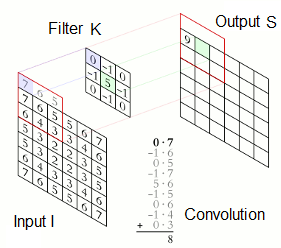
\includegraphics{img/faltung2.png}
			\captionof{figure}{Faltung einer 6x6 Matrix mit einem 3x3 Filter \cite{wikipic}}
			\label{img:faltung}
		\end{minipage}\newline
		\subsubsection*{Convolutional Layer}
		In einem CL findet eine Faltung der Eingangsdaten, in Form einer Matrix, und einem oder mehreren Filtern statt. Ein Filter dient beispielsweise zur Glättung oder zur Verkleinerung der Daten. Eine Verkleinerung der Eingangsmatrix findet statt, wenn ein Filter ohne Zero-padding\footnote[11]{Eine Matrix wird am Rand um Nullen erweitert.\\ Bsp. aus einer 7x7 Matrix wird eine 9x9 Matrix} verwendet wird. Die Parameter eines Filters werden zufällig initialisiert, können aber mit Hilfe des Backpropagation Verfahren (3.1.2) angepasst werden. Werden mehrere Filter auf die Eingangsdaten angewendet, ändert sich die Tiefe der gesamten Ausgangsmatrix entsprechend der Anzahl der Filter. \cite{karpathy}\newline
		In Abbildung \ref{img:faltung} ist die Eingabematrix \textit{I} eine 6x6 Matrix und \textit{K} ein 3x3 Filter. Die Ausgabematrix \textit{S} wir an den Stellen (i,j) durch die nachfolgende Gleichung berechnet. Eine genauere Herleitung der Gleichung findet der Leser u. a. bei \cite{goodfellow}(328f).\newline\\	
		\begin{equation*}
		S(i,j) =(I \star K)(i,j)
		\end{equation*}
		\begin{equation*}
		(I \star K)(i,j) =\newline\sum_{m}^{}\sum_{n}^{}I(i+m,j+n)K(m,n)
		\end{equation*}\newline\\
		\subsubsection*{Pooling Layer}
		Ein PL wird zwischen zwei CL eingefügt. Ihre Funktion besteht darin, die Größe der Daten zu reduzieren und damit die Anzahl der Parameter für das nächste CL. Durch die Reduzierung wird die Berechnung des gesamten Netzwerkes beschleunigt. \cite{karpathy}\newline Ein PL wandelt die Ausgabe eines CL, durch eine statistische Zusammenfassung von nebeneinander liegenden Ausgängen um. Verschiedene Methoden für ein Pl sind: Max Pooling \cite{zhou}, eine Übergabe der größten Zahl in einem rechteckigen Umfeld; die Durchschnittsberechnung des Umfeldes oder ein gewichteter Durchschnitt basierend auf der Entfernung eines zentralen Punktes \cite{goodfellow}(355).\newline
		Abbildung \ref{img:pooling} zeigt einen 2x2 Max-Filter, der auf eine 4x4 Datenmatrix angewandt wird. Die Verschiebung oder Stride des Filters ist 2 dh. der Filter wird zunächst auf der y-Achse verschoben. Erreicht er dort das Ende wird er um eine Stride auf der x-Achse verschoben und beginnt wieder mit der y-Verschiebung.\newline\\
		\begin{minipage}{0.4\textwidth}
			\centering
			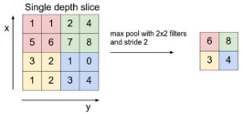
\includegraphics{img/pooling.png}
			\captionof{figure}{Maxpooling mit einem 2x2 Filter\cite{karpathy}}
			\label{img:pooling}
		\end{minipage}\newline
		\subsubsection*{Fully-Connected Layer}
		Ein oder mehrere geschachtelte FCL dienen bei einem Klassifizierungsproblem aus Ausgabeschicht. Die Anzahl der Knoten in der letzten FCL entsprechen der Anzahl der Klassen, die das CNN unterscheiden soll.
		Jeder Knoten in einer FCL hat eine Verbindungen zu allen Knoten der vorherigen Schicht. Die Ausgabe der FCL ist ein Vektor, in der jeder Eintrag die Wahrscheinlichkeit der jeweiligen Klasse spiegelt. \cite{karpathy}
		\subsubsection{Training}
		CNNs werden durch die Backpropagation Methode trainiert. Backpropagation basiert auf dem Gradientenverfahren, welches versucht für die Fehlerfunktion \textit{E}, durch sukzessive Iteration der Parameter ein globales Minimum zu finden, meistens aber nur ein lokales findet. Um das Minimum zu erreichen, werden die Werte der Gewichte \textit{w}\textsubscript{ij} durch Verwendung der Kettenregel, der partiellen Ableitung, berechnet:\footnote[12]{Ausgabeparameter \textit{o}, beliebige Anzahl an Knoten \textit{net} zwischen Ausgabe und \textit{w}}
		\begin{equation*}
		\centering
		\frac{\partial\textit{E}}{\partial\textit{w}\textsubscript{ij}} = \frac{\partial\textit{E}}{\partial\textit{o}\textsubscript{j}} \frac{\partial\textit{o}\textsubscript{j}}{\partial\textit{net}\textsubscript{j}}  \frac{\partial\textit{net}\textsubscript{j}}{\partial\textit{w}\textsubscript{ij}} 
		\end{equation*}\newline
		Der neue Wert eines Parameters \textit{w} zum Zeitpunkt \textit{t} lässt sich dann durch die folgende Formel berechnen:
		\begin{equation*}
		\centering
		\textit{w}(\textit{t}) = \textit{w}(\textit{t}-1) + \eta * \frac{\partial\textit{E}}{\partial\textit{w}} 
		\end{equation*}
		Die Lernrate $\eta$ ist eine Konstante die definiert werden muss.\newline
		Anhand der Kostenfunktion, kann die Parameteranpassung und damit der funktionale Wert eines CNN mit reellen Zahlen dargestellt und verglichen werden. Diese Funktion \textit{C} lässt sich durch die Summe über Trainingsbeispiele \textit{m} und einer Fehlerfunktion \textit{E}, hier die negativ conditional Log-Likelihood\footnote[13]{Abgeleitet von Maximum Likelihood, Dichtefunktion für Maximafindung} darstellen: 
		\begin{equation*}
			\centering
			E(x,y) = -log p(y|x)
		\end{equation*}
		\begin{equation*}
			\centering
			\textit{C} = \frac{1}{m}\sum_{i=1}^{m}E(x\textsuperscript{i},y\textsuperscript{i})
		\end{equation*}
		Das Training eines Netzes ist abgeschlossen, wenn die Kostenfunktion minimal ist bzw. wenn in einem gegebenen Zeitraum keine bessere Kostenfunktion gefunden wird. \cite{goodfellow}(80ff,129ff)
		\subsection{Musikempfehlung mit Neuronalen Netzwerken}
		\subsubsection*{Anwendung eines CNN zur automatischen Musikempfehlung}
		\subsection{Hybride Musikempfehlung mit einem Neuronalen Netzwerk}
		Im Unterschied zu der zuvor dargestellten Forschung (3.2) wird in der jetzigen ein Deep Belief Netzwerk(DBN) verwendet, um ein hybrides inhaltsbasiertes Musikempfehlungssystem zu entwickeln. Bisherige inhaltsbasiertes Systeme verfolgen typischerweise einem zweistufigen Ansatz: zunächst extrahieren sie aus Audioinhalte den MFCC Koeffizienten; anschließend prognostizieren sie Musikpräferenzen eines Nutzers. Das nachfolgende Modell führt dieses beiden Schritte simultan und automatisch aus. \cite{wang}\newline
		Das hybride Modell basiert auf einem hierarchischen linearen Modell mit einem Deep Belief Netzwerk(HLDBN), dass zunächst erläutert wird, um anschließend die Funktionsweise des hybriden Systems darzustellen.
		\begin{minipage}{0.45\textwidth}
			\centering
			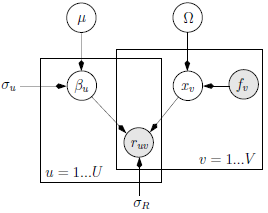
\includegraphics{img/hlmdbn.png}
			\captionof{figure}{Hierarchisches lineares Modell eins Deep Belief Netzwerks \cite{wang}}
			\label{img:hlmdbn}
		\end{minipage}
		\subsubsection{Hierarchisches lineares Modell mit einem Deep Belief Netzwerk}
		Das in Abbildung \ref{img:hlmdbn} gezeigte Modell ist wie folgt definiert: \textit{f\textsubscript{v}} sind Musikmerkmale eines Liedes \textit{v}, die durch den Merkmalsvektor x\textsubscript{v} automatisch errechnet werden. Die bevorzugte Musik eines Benutzers \textit{u} wird as Vektor $\beta$\textsubscript{u} bezeichnet. $\Omega$ bezeichnet die Parameter, die das DBN lernt. Die Bewertung \textit{r\textsubscript{xv}}, die ein Nutzer einem Lied \textit{v} gibt, ist ein Skalarprodukt von \textit{x\textsubscript{v}} und $\beta$\textsubscript{u}. Durch $\sigma$\textsubscript{R} wird die Varianz aller Bewertungen des Nutzers betrachtet. $\mu$ repräsentiert den allgemeinen Musikgeschmack aller Benutzer, wobei $\sigma$\textsubscript{u} die Varianz des einzelnen Nutzers definiert. Alle Benutzer und Lieder Paare werden als \textit{I} bezeichnet. Für eine Regularisierung der Werte wird die Gaußsche Normalverteilung $\mathcal{N}$ verwenden.\footnote[14]{$\mathcal{N}$(a,b) ist die Normalverteilung mit Mittelwert a und Varianz b. x $\sim$ p zeigt, dass x die Verteilung p erfüllt} \cite{wang}\newline Das Modell ist wie folgt formuliert:\newline
		\begin{equation*}
			\centering
			\textit{r\textsubscript{xv}}\sim\mathcal{N}(\beta'\textit{x\textsubscript{v}},\sigma\textsuperscript{2}\textsubscript{R})
		\end{equation*}
		\begin{equation*}
		\centering
			\beta\sim\mathcal{N}(\mu,\sigma\textsuperscript{2}\textsubscript{u}\textit{I})
		\end{equation*}
		\begin{equation*}
			\textit{x\textsubscript{v}} = DBN(\textit{f\textsubscript{v}};\Omega)
		\end{equation*}\newline\\
		Für das Training des Systems wird im Unterschied zu einem CNN zunächst ein unsupervised\footnote[15]{Ausgabeergebnisse der Testdaten sind nicht vorhanden} Training durchgeführt um die Knoten zu initialisieren. Anschließend findet ein supervised Training zur Optimierung der Parameter statt. Als Optimierungsmethode wird das stochastische Mini-Batch\footnote[16]{nur ein kleiner Teil der vorhandenen Daten wird trainiert} Verfahren mit Backpropagation genutzt, um ein Overfitting\footnote[17]{Spezialisierung} des Modells zu vermeiden. Nach der Lernphase kann die Bewertung \textit{r\textsubscript{xv}} eines Benutzers \textit{u} über ein Lied \textit{v} geschätzt werden, wodurch diesem neue Lieder empfohlen werden können. \cite{wang}
		\subsubsection{Hybrides Modell mit einem Deep Belief Netzwerk}
		Basiert auf dem HLDBM wird das in Abbildung \ref{img:hybrid} gezeigte Modell um einen kollaborative Filter erweitert, um eine noch bessere Empfehlungsrate zu erhalten.
		\begin{minipage}{0.45\textwidth}
			\centering
			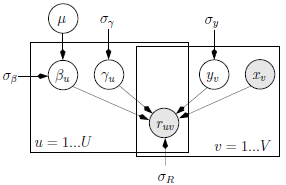
\includegraphics{img/hybrid.png}
			\captionof{figure}{Hybrides Empfehlungs Modell \cite{wang}}
			\label{img:hybrid}
		\end{minipage}\newline\\
		Die Musikmerkmale eines Liedes \textit{x}\textsubscript{v} und die bevorzugte Musik eines Nutzers $\beta$\textsubscript{u} werden wie in (3.4.1) berechnet. $\gamma$\textsubscript{u} stellt einen Merkmalsvektor eines Benutzers \textit{u}; \textit{y}\textsubscript{v} den Merkmalsvektor eines Liedes \textit{v} dar. $\beta$\textsubscript{u}, $\gamma$\textsubscript{u} und \textit{y}\textsubscript{v} werden durch das Neuronale Netzwerk anhand der Trainingsdaten gelernt. Die Empfehlungsrate \textit{r}\textsubscript{uv} ergibt sich aus der Summe der Skalarmultiplikationen  $\gamma$'\textsubscript{u}\textit{y}\textsubscript{v} und  $\beta$'\textsubscript{u}\textit{x}\textsubscript{v}. Die A-priori-Wahrscheinlichkeit\footnote[18]{Anfangswahrscheinlichkeit} werden durch die folgenden Formeln definiert:\newline
		\begin{equation*}
		\centering
		\textit{r\textsubscript{xv}}|\beta\textsubscript{u},\textit{x}\textsubscript{v},\gamma\textsubscript{u},\textit{y}\textsubscript{v},\sigma\textsubscript{R}\sim\mathcal{N}(\beta'\textsubscript{u}\textit{x}\textsubscript{v} + \gamma'\textsubscript{u}\textit{y}\textsubscript{v},\sigma\textsubscript{R}\textsuperscript{2})
		\end{equation*}
		\begin{equation*}
		\centering
		\beta\textsubscript{u}|\sigma\textsubscript{$\beta$}\sim\mathcal{N}(\mu,|\sigma\textsubscript{$\beta$}\textsuperscript{2}I)
		\end{equation*}
		\begin{equation*}
		\centering
		\gamma\textsubscript{u}|\sigma\textsubscript{u}\sim\mathcal{N}(0,|\sigma\textsubscript{$\gamma$}\textsuperscript{2})
		\end{equation*}
		\begin{equation*}
		\centering
		\textit{y}\textsubscript{v}|\sigma\textsubscript{v}\sim\mathcal{N}(0,|\sigma\textsubscript{y}\textsuperscript{2})
		\end{equation*}\newline
		Die Fehler Funktion des Modells wird auch mit Hilfe der Backpropagation minimiert. Alternative können  die Werte für $\gamma$\textsubscript{u} und \textit{y}\textsubscript{v} durch eine PMF berechnet und als Initialwerte verwendet werden.
		\section{Vergleich der vorgestellten Modelle}
		Abschließend wird nun ein Vergleich zwischen dem vorgestellten CNN Ansatz einerseits und dem danach folgendem DBN gezogen. In Versuchen \cite{oord} wurde festgestellt das dass CNN Model einem BOW System überlegen ist und eine bessere Empfehlungsrate erreicht. Das anschließend erläuterte  Versuchsmodel, welches mittels DBN einen hybriden Methode verfolgt, konnte im direkten Vergleich zu CNN eine nochmals verbesserte Empfehlungsgenauigkeit erreichen. Vergleichende Versuchsreihen \cite{wang} haben folgendes festgestellt: ein nicht hybrider Ansatz welcher allein auf Training der beiden Netze ergab, dass das vorgestellte HLDBN Modell genauere Ergebnisse lieferte als das vorgestellte CNN. Die integration der beiden Modelle in einen hybriden Aufbau ergab wiederum ebenso dass der Einsatz des HLDBN Netzes zu genaueren Empfehlungsraten führte als die Verknüpfung von CNN und CF. Die Empfehlungsraten für bereits bekannte Lieder, konnten somit im Vergleich zu klassischen Ansätzen verbessert werden. Auch das bereits eingeführte Problem des NSP konnte durch den Einsatz Neuronaler Netze gelöst werden.  Sowohl der Einsatz des CNN als auch der des HLDBN Netzes führen hierbei zum Erfolg.
		Sowohl der im Punkt 3.2 vorgestellte ansatz mittels eines CNNs sowie der in Punkt 3.3 erläuterte Ansatz mit Einsatz eines hybriden dbn Netzwerkes eine gute Möglichkeit zur automatisierten Musikempfehlung. Beide Verfahren haben in Rahmen von Versuchen bewiesen, dass sie sowohl zuverlässig sind, aber auch das sie einen klassisches Verfahren wie ein BoW-System 
		%\bibliographystyle{abbrvdin}
		\bibliographystyle{unsrt}
		\bibliography{lit}
	\end{multicols}
\end{document}
